% Options for packages loaded elsewhere
\PassOptionsToPackage{unicode}{hyperref}
\PassOptionsToPackage{hyphens}{url}
%
\documentclass[
  12pt,
  a4paper,
  DIV=11,
  numbers=noendperiod]{scrreprt}

\usepackage{amsmath,amssymb}
\usepackage{setspace}
\usepackage{iftex}
\ifPDFTeX
  \usepackage[T1]{fontenc}
  \usepackage[utf8]{inputenc}
  \usepackage{textcomp} % provide euro and other symbols
\else % if luatex or xetex
  \usepackage{unicode-math}
  \defaultfontfeatures{Scale=MatchLowercase}
  \defaultfontfeatures[\rmfamily]{Ligatures=TeX,Scale=1}
\fi
\usepackage{lmodern}
\ifPDFTeX\else  
    % xetex/luatex font selection
    \setmainfont[Ligatures=TeX]{PT Serif}
    \setsansfont[Ligatures=TeX,Scale=MatchLowercase]{PT Sans}
    \setmonofont[Scale=MatchLowercase,Scale=0.9]{PT Mono}
\fi
% Use upquote if available, for straight quotes in verbatim environments
\IfFileExists{upquote.sty}{\usepackage{upquote}}{}
\IfFileExists{microtype.sty}{% use microtype if available
  \usepackage[]{microtype}
  \UseMicrotypeSet[protrusion]{basicmath} % disable protrusion for tt fonts
}{}
\usepackage{xcolor}
\setlength{\emergencystretch}{3em} % prevent overfull lines
\setcounter{secnumdepth}{5}
% Make \paragraph and \subparagraph free-standing
\makeatletter
\ifx\paragraph\undefined\else
  \let\oldparagraph\paragraph
  \renewcommand{\paragraph}{
    \@ifstar
      \xxxParagraphStar
      \xxxParagraphNoStar
  }
  \newcommand{\xxxParagraphStar}[1]{\oldparagraph*{#1}\mbox{}}
  \newcommand{\xxxParagraphNoStar}[1]{\oldparagraph{#1}\mbox{}}
\fi
\ifx\subparagraph\undefined\else
  \let\oldsubparagraph\subparagraph
  \renewcommand{\subparagraph}{
    \@ifstar
      \xxxSubParagraphStar
      \xxxSubParagraphNoStar
  }
  \newcommand{\xxxSubParagraphStar}[1]{\oldsubparagraph*{#1}\mbox{}}
  \newcommand{\xxxSubParagraphNoStar}[1]{\oldsubparagraph{#1}\mbox{}}
\fi
\makeatother


\providecommand{\tightlist}{%
  \setlength{\itemsep}{0pt}\setlength{\parskip}{0pt}}\usepackage{longtable,booktabs,array}
\usepackage{calc} % for calculating minipage widths
% Correct order of tables after \paragraph or \subparagraph
\usepackage{etoolbox}
\makeatletter
\patchcmd\longtable{\par}{\if@noskipsec\mbox{}\fi\par}{}{}
\makeatother
% Allow footnotes in longtable head/foot
\IfFileExists{footnotehyper.sty}{\usepackage{footnotehyper}}{\usepackage{footnote}}
\makesavenoteenv{longtable}
\usepackage{graphicx}
\makeatletter
\def\maxwidth{\ifdim\Gin@nat@width>\linewidth\linewidth\else\Gin@nat@width\fi}
\def\maxheight{\ifdim\Gin@nat@height>\textheight\textheight\else\Gin@nat@height\fi}
\makeatother
% Scale images if necessary, so that they will not overflow the page
% margins by default, and it is still possible to overwrite the defaults
% using explicit options in \includegraphics[width, height, ...]{}
\setkeys{Gin}{width=\maxwidth,height=\maxheight,keepaspectratio}
% Set default figure placement to htbp
\makeatletter
\def\fps@figure{htbp}
\makeatother

\KOMAoption{captions}{tableheading}
\usepackage{indentfirst}
\usepackage{float}
\floatplacement{figure}{H}
\usepackage{libertine}
\usepackage{indentfirst}
\usepackage{float}
\floatplacement{figure}{H}
\makeatletter
\@ifpackageloaded{caption}{}{\usepackage{caption}}
\AtBeginDocument{%
\ifdefined\contentsname
  \renewcommand*\contentsname{Содержание}
\else
  \newcommand\contentsname{Содержание}
\fi
\ifdefined\listfigurename
  \renewcommand*\listfigurename{Список иллюстраций}
\else
  \newcommand\listfigurename{Список иллюстраций}
\fi
\ifdefined\listtablename
  \renewcommand*\listtablename{Список таблиц}
\else
  \newcommand\listtablename{Список таблиц}
\fi
\ifdefined\figurename
  \renewcommand*\figurename{Рисунок}
\else
  \newcommand\figurename{Рисунок}
\fi
\ifdefined\tablename
  \renewcommand*\tablename{Таблица}
\else
  \newcommand\tablename{Таблица}
\fi
}
\@ifpackageloaded{float}{}{\usepackage{float}}
\floatstyle{ruled}
\@ifundefined{c@chapter}{\newfloat{codelisting}{h}{lop}}{\newfloat{codelisting}{h}{lop}[chapter]}
\floatname{codelisting}{Список}
\newcommand*\listoflistings{\listof{codelisting}{Листинги}}
\makeatother
\makeatletter
\makeatother
\makeatletter
\@ifpackageloaded{caption}{}{\usepackage{caption}}
\@ifpackageloaded{subcaption}{}{\usepackage{subcaption}}
\makeatother

\ifLuaTeX
\usepackage[bidi=basic]{babel}
\else
\usepackage[bidi=default]{babel}
\fi
\babelprovide[main,import]{russian}
\ifPDFTeX
\else
\babelfont{rm}[Ligatures=TeX]{PT Serif}
\fi
\babelprovide[import]{english}
% get rid of language-specific shorthands (see #6817):
\let\LanguageShortHands\languageshorthands
\def\languageshorthands#1{}
\ifLuaTeX
  \usepackage{selnolig}  % disable illegal ligatures
\fi
\usepackage[style=gost-numeric,parentracker=true,backend=biber,hyperref=auto,language=auto,autolang=other*,citestyle=gost-numeric]{biblatex}
\addbibresource{bib/cite.bib}
\usepackage{csquotes}
\usepackage{bookmark}

\IfFileExists{xurl.sty}{\usepackage{xurl}}{} % add URL line breaks if available
\urlstyle{same} % disable monospaced font for URLs
\hypersetup{
  pdftitle={Отчёт по лабораторной работе №4},
  pdfauthor={Герчет Вячеслав, группа НКАбд-03-25},
  pdflang={ru-RU},
  hidelinks,
  pdfcreator={LaTeX via pandoc}}


\title{Отчёт по лабораторной работе №4}
\usepackage{etoolbox}
\makeatletter
\providecommand{\subtitle}[1]{% add subtitle to \maketitle
  \apptocmd{\@title}{\par {\large #1 \par}}{}{}
}
\makeatother
\subtitle{Создание и процесс обработки программ на языке ассемблера
NASM}
\author{Герчет Вячеслав, группа НКАбд-03-25}
\date{}

\begin{document}
\maketitle

\renewcommand*\contentsname{Содержание}
{
\setcounter{tocdepth}{1}
\tableofcontents
}
\listoffigures
\listoftables

\setstretch{1.5}
\chapter{Цель
работы}\label{ux446ux435ux43bux44c-ux440ux430ux431ux43eux442ux44b}

Освоить процесс компиляции и сборки программ на языке ассемблера NASM,
научиться использовать транслятор NASM и компоновщик LD, а также
закрепить практические навыки работы с файлами исходного кода и
объектными файлами.

\chapter{Задание}\label{ux437ux430ux434ux430ux43dux438ux435}

Написать две программы: 1. Программа \textbf{Hello world} --- вывод
текста на экран. 2. Программа \textbf{lab4.asm} --- аналогичная, но с
персонализированным выводом \enquote{Герчет Вячеслав}.

\chapter{Выполнение лабораторной
работы}\label{ux432ux44bux43fux43eux43bux43dux435ux43dux438ux435-ux43bux430ux431ux43eux440ux430ux442ux43eux440ux43dux43eux439-ux440ux430ux431ux43eux442ux44b}

\section{Программа Hello
world!}\label{ux43fux440ux43eux433ux440ux430ux43cux43cux430-hello-world}

Создать файл hello.asm и написать код, выводящий строку \enquote*{Hello
world!}. на языке ассемблера NASM (рис. \textcite{fig:001}).

\begin{figure}

{\centering 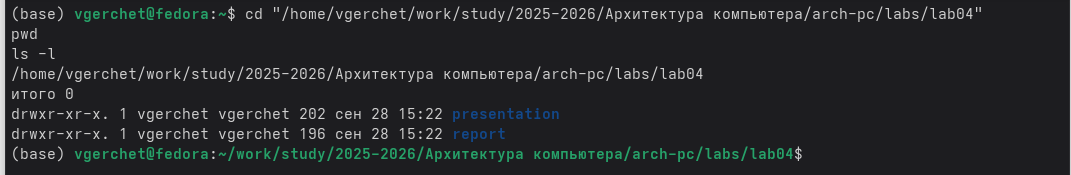
\includegraphics[width=0.7\textwidth,height=\textheight]{image/1.png}

}

\caption{Переход в каталог лабораторной работы №4}

\end{figure}%

с помощью команды gedit открыл редакторе (рис. \textcite{fig:002}).

\begin{figure}

{\centering 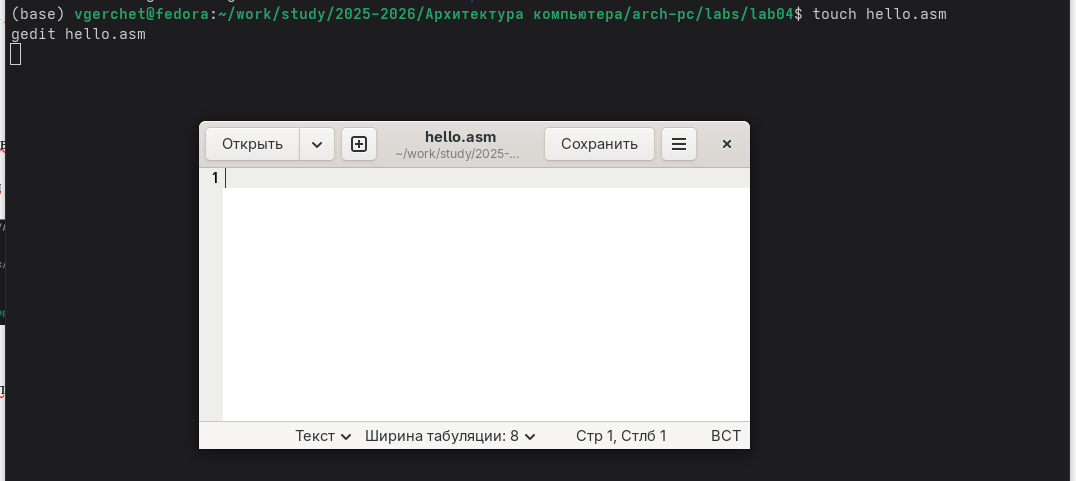
\includegraphics[width=0.7\textwidth,height=\textheight]{image/2.png}

}

\caption{с помощью команды gedit открыл редакторе}

\end{figure}%

исходный код программы hello.asm (рис. \textcite{fig:003}).

\begin{figure}

{\centering 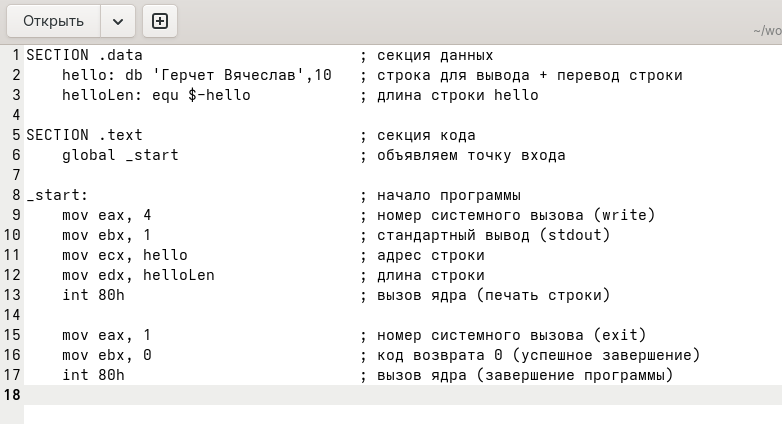
\includegraphics[width=0.7\textwidth,height=\textheight]{image/3.png}

}

\caption{исходный код программы hello.asm}

\end{figure}%

\section{Транаслятор
NASM}\label{ux442ux440ux430ux43dux430ux441ux43bux44fux442ux43eux440-nasm}

Трансляция исходного файла hello.asm в объектный файл hello.o (рис.
\textcite{fig:004}).

\begin{figure}

{\centering 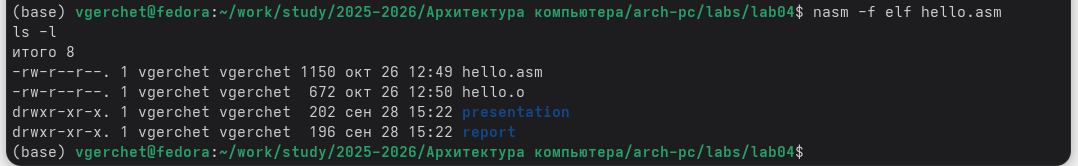
\includegraphics[width=0.7\textwidth,height=\textheight]{image/4.png}

}

\caption{Используем команду nasm и сразу все проверяем.}

\end{figure}%

\section{Расширенный синтаксис командной строки
NASM}\label{ux440ux430ux441ux448ux438ux440ux435ux43dux43dux44bux439-ux441ux438ux43dux442ux430ux43aux441ux438ux441-ux43aux43eux43cux430ux43dux434ux43dux43eux439-ux441ux442ux440ux43eux43aux438-nasm}

Компилируем исходный файл (рис. \textcite{fig:005}).

\begin{figure}

{\centering 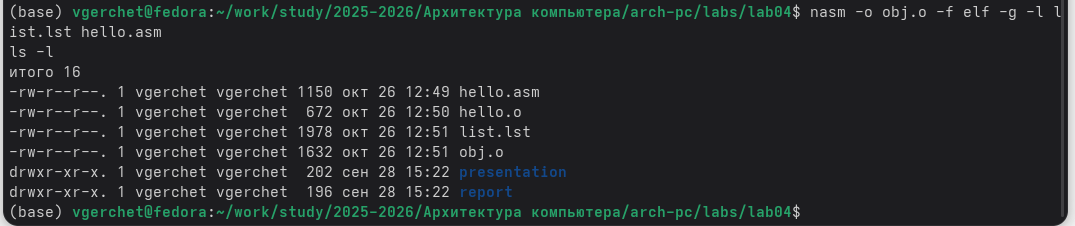
\includegraphics[width=0.7\textwidth,height=\textheight]{image/5.png}

}

\caption{Преобразуем файл hello.asm в obj.o}

\end{figure}%

\section{Компоновщик
LD}\label{ux43aux43eux43cux43fux43eux43dux43eux432ux449ux438ux43a-ld}

Выполнить компоновку: ld -m elf\_i386 hello.o -o hello. (рис.
\textcite{fig:006}).

\begin{figure}

{\centering 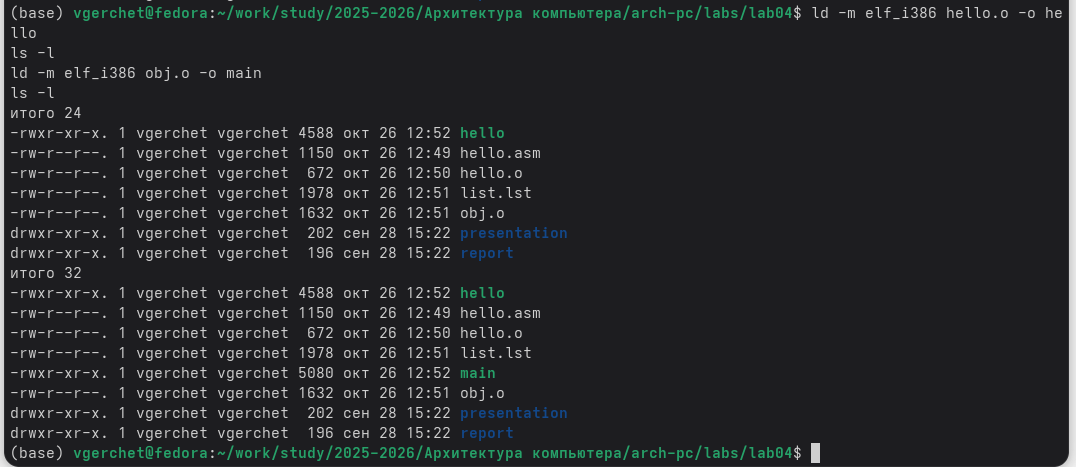
\includegraphics[width=0.7\textwidth,height=\textheight]{image/6.png}

}

\caption{Компоновка объектных файлов в исполняемые файлы hello и main}

\end{figure}%

\section{Запуск исполняемого
файла}\label{ux437ux430ux43fux443ux441ux43a-ux438ux441ux43fux43eux43bux43dux44fux435ux43cux43eux433ux43e-ux444ux430ux439ux43bux430}

Запускаем на выполнение созданный исполняемый файл (рис.
\textcite{fig:07}).

\begin{figure}

{\centering 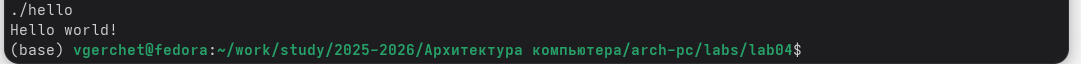
\includegraphics[width=0.7\textwidth,height=\textheight]{image/7.png}

}

\caption{Используем команду ./hello}

\end{figure}%

\section{Задание для самостоятельной
работы}\label{ux437ux430ux434ux430ux43dux438ux435-ux434ux43bux44f-ux441ux430ux43cux43eux441ux442ux43eux44fux442ux435ux43bux44cux43dux43eux439-ux440ux430ux431ux43eux442ux44b}

Создать копию hello.asm под именем lab4.asm, изменить текст на
\enquote*{Герчет Вячеслав}, выполнить трансляцию, компоновку и запуск.
(рис. \textcite{fig:08}).

\begin{figure}

{\centering 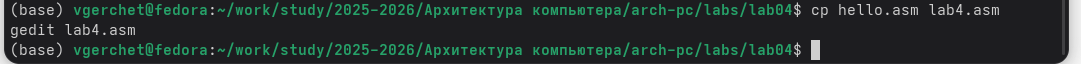
\includegraphics[width=0.7\textwidth,height=\textheight]{image/8.png}

}

\caption{открываю редактор}

\end{figure}%

меняю текст на hello: db \enquote*{Герчет Вячеслав},10 (рис.
\textcite{fig:09}).

\begin{figure}

{\centering 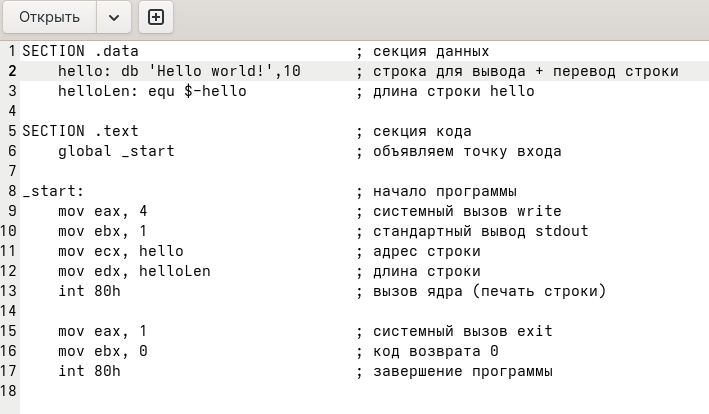
\includegraphics[width=0.7\textwidth,height=\textheight]{image/9.png}

}

\caption{в текстовом редакторе редактирую 2 линию}

\end{figure}%

Компоновка объектного файла в исполняемый файл, запуск программы
lab4.asm с персонализированным выводом. (рис. \textcite{fig:010}).

\begin{figure}

{\centering 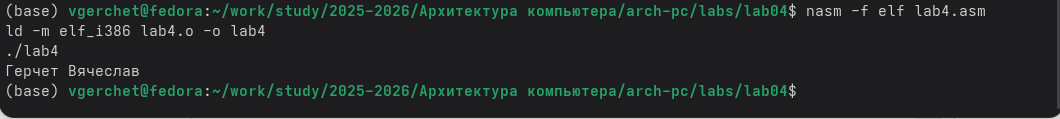
\includegraphics[width=0.7\textwidth,height=\textheight]{image/10.png}

}

\caption{Прописываем команды для работы файла и запускаем программу}

\end{figure}%

Переходим в каталог лабораторных работ и загружаем файлы на Github (рис.
\textcite{fig:011}).

\begin{figure}

{\centering 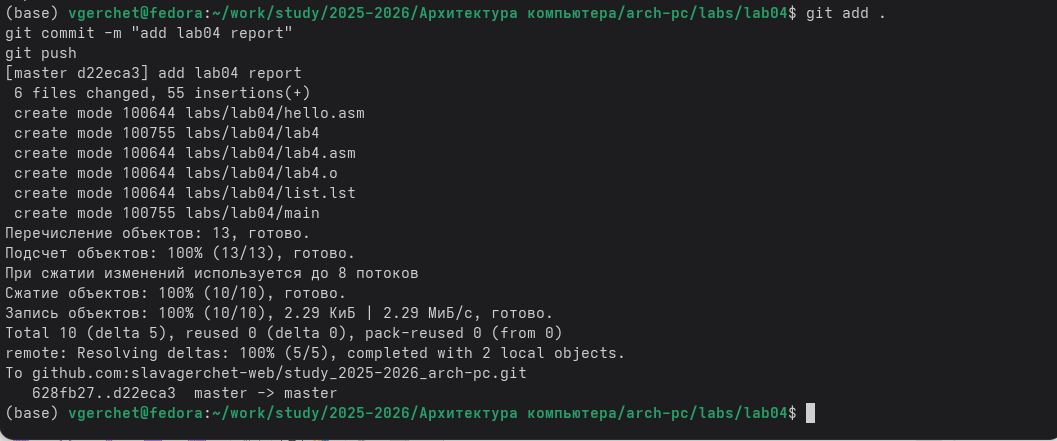
\includegraphics[width=0.7\textwidth,height=\textheight]{image/11.png}

}

\caption{Загружаем файлы}

\end{figure}%

\chapter{Выводы}\label{ux432ux44bux432ux43eux434ux44b}

Мы познакомились с языком ассемблера NASM и создали две работающих
программы.


\printbibliography



\end{document}
